\documentclass[border=10pt]{standalone}

\usepackage{tikz}
\usepackage{tikzsymbols}
\usetikzlibrary{calc,patterns,shapes.geometric}

\def\centerarc[#1](#2)(#3:#4:#5){\draw[#1] ($(#2)+({#5*cos(#3)},{#5*sin(#3)})$) arc (#3:#4:#5);}

\begin{document}
	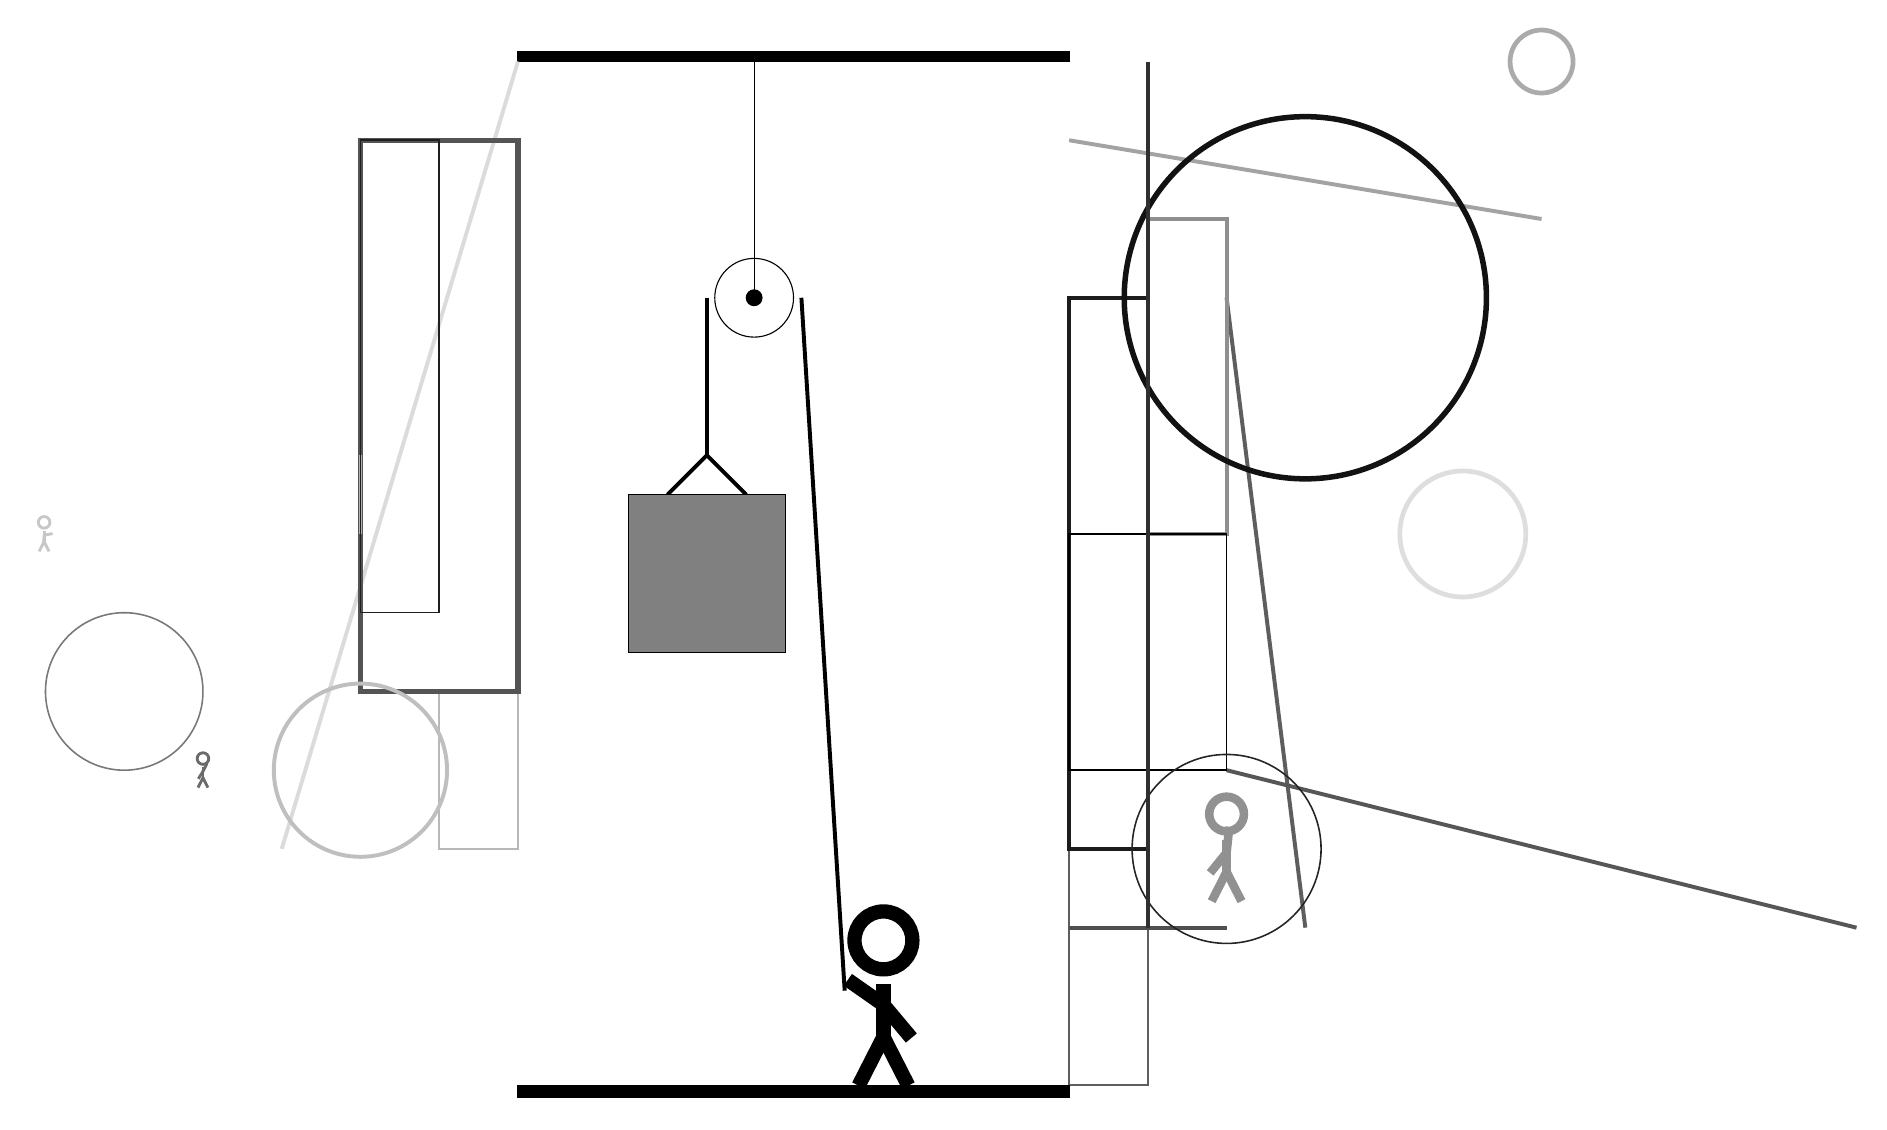
\begin{tikzpicture}
		%%%%% START %%%%%
		
		\draw[fill=black] (-2, 10) rectangle (5, 10.125);
		
		\draw (1, 7) circle (0.5);
		\draw[fill=black] (1, 7) circle (0.1);
		\draw (1, 10) -- (1, 7);
		
		\draw[line width=0.5mm] (-0.1, 4.5) -- (0.4, 5.0) -- (0.9, 4.5);
		\draw[fill=black!50] (-0.6, 4.5) rectangle (1.4, 2.5);
		
		\draw[line width=0.5mm] (0.4, 7) -- (0.4, 5.0);
		\centerarc[line width=0.5mm](1, 7)(0:180:0.6);
		\draw[line width=0.5mm](1.6, 7) -- (2.15, -1.8);
		
		\draw[line width=0.2mm, color=black!28] (-2, 0) rectangle (-3, 2);
		
		\draw[line width=0.2mm, color=black!63] (6, 0) rectangle (5, -3);
		\node[line width=0.3mm, color=black!58] at (-6, 1) {\Strichmaxerl[2][58][63]};
		\draw [line width=0.6mm, color=black!33](11, 10) circle (0.4);
		\draw[line width=0.5mm, color=black!14](-2, 10) -- (-5, 0);
		\draw [line width=0.6mm, color=black!13](10, 4) circle (0.8);
		\draw[line width=0.5mm, color=black!36](5, 9) -- (11, 8);
		\draw[line width=0.5mm, color=black!63](7, 7) -- (8, -1);
		\draw[line width=0.7mm, color=black!67] (-2, 9) rectangle (-4, 2);
		
		\draw[line width=0.5mm, color=black!44] (6, 8) rectangle (7, 4);
		
		\draw[line width=0.5mm, color=black!66](7, 1) -- (15, -1);
		
		\draw[line width=0.5mm, color=black!69](5, -1) -- (7, -1);
		\draw[line width=0.5mm, color=black!89] (6, 0) rectangle (5, 7);
		
		\node[line width=0.6mm, color=black!43] at (7, 0) {\Strichmaxerl[6][51][84]};
		\draw[line width=0.2mm, color=black!100] (7, 4) rectangle (5, 1);
		\draw[line width=0.3mm, color=black!30] (-4, 5) rectangle (-4, 4);
		\draw [line width=0.7mm, color=black!93](8, 7) circle (2.3);
		\draw [line width=0.2mm, color=black!53](-7, 2) circle (1.0);
		\draw [line width=0.5mm, color=black!25](-4, 1) circle (1.1);
		\draw[line width=0.2mm, color=black!88] (-4, 9) rectangle (-3, 3);
		\node[line width=0.3mm, color=black!22] at (-8, 4) {\Strichmaxerl[2][86][11]};
		
		\draw [line width=0.2mm, color=black!86](7, 0) circle (1.2);
		
		\draw[line width=0.5mm, color=black!81](6, 10) -- (6, -1);
		
		\node at (2.6, -1.9) {\Strichmaxerl[10][-35][-50]};
		
		\draw[fill=black] (-2, -3) rectangle (5, -3.15);
		
		%%%%% END %%%%%
	\end{tikzpicture}
\end{document}